e) Escribir un programa que acepte un apuntador a un
árbol binario y retorne un apuntador a un nuevo árbol
binario que sea la imagen reflejo del primero, es decir,
que todos los subárboles izquierdos sean ahora subárboles
derechos y viceversa.
\lstinputlisting{Arboles/TareaE.c}
Capturas de Pantalla de Arboles/TareaE.c
\newline
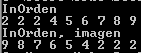
\includegraphics{Arboles/img/TareaE_1.png}